\documentclass[xcolor=dvipsnames]{beamer}
\usecolortheme[named=Brown]{structure}
\usetheme{default}
\setbeamertemplate{navigation symbols}{} 
\usepackage{tikz}
\usetikzlibrary{arrows,decorations.pathmorphing,backgrounds,positioning,fit}
\usetikzlibrary{datavisualization.formats.functions}
\include{macro}
\usepackage{epsfig}
\begin{document}
%\setbeamercolor{titlelike}{fg=gray,bg=white}
%\setbeamercolor{itemize item}{fg=gray,bg=white}
%\setbeamercolor{enumerate item}{fg=gray,bg=white}
%\setbeamercolor{block title}{fg=black,bg=white}
%==============================================
\title{Full Waveform Inversion in the data and image space}
\author{W. Weibull and B. Arntsen}
\institute[NTNU]{
  NTNU\\
  Department of Petr. Techn. and Applied Geophysics\\
  \texttt{borge.arntsen@ntnu.no}
}
\date{EAGE June 7, 2012}
\begin{frame}
 \titlepage
\end{frame}
%==============================================
%-----------------------------------------
\begin{frame}{Overview}
%-----------------------------------------
\begin{enumerate}
  \item Introduction
  \item Initial models for FWI
  \item Wave Equation Migration Velocity Analysis
  \item Joint Inversion in the image and data spaces
  \item Numerical Example
  \item Conclusions
\end{enumerate}
\end{frame}
%-----------------------------------------
\begin{frame}{Introduction}
%-----------------------------------------
\center{Full Waveform Inversion loop}
\begin{figure}
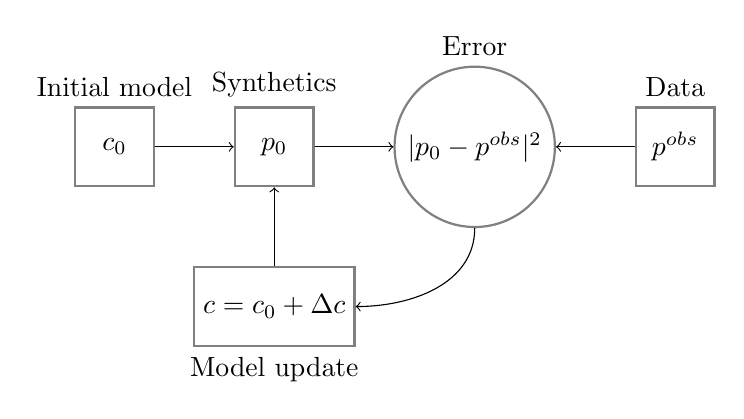
\begin{tikzpicture}
[place/.style={rectangle,draw=black!50,fill=white!20,thick,minimum size=10mm}]
\node[place] (parameter) [label=above:Initial model]{$c_0$};
\node[place] (modeling) [right=of parameter,label=above:Synthetics] {$p_0$};
\node[circle,draw=black!50,fill=white!20,thick,minimum size=10mm] (error) 
    [right=of modeling,label=above:Error] {$|p_0-p^{obs}|^2$};
\node[place] (data) [right=of error,label=above:Data] {$p^{obs}$};
\node[place] (update) [below=of modeling,label=below:Model update] {$c=c_0+\Delta c$};
\draw[->](parameter) -- (modeling);
\draw[->](modeling) -- (error);
\draw[->](data) -- (error);
\draw[->](error) to [out=270,in=0] (update);
\draw[->](update) -- (modeling);
\end{tikzpicture}
\end{figure}
\end{frame}
%-----------------------------------------
\begin{frame}{Introduction}
%-----------------------------------------
Full Waveform Inversion (FWI) 
minimization the least-squares error w.r.t. velocity (Tarantola, 1984) 
\begin{eqnarray}
  e_l = |p-p^{obs}|^2
\end{eqnarray}
Linearization leads to a Newton-Raphson Scheme
where the first iteration is
\begin{eqnarray}
  \JJ^T [p_0-p^{obs}]= \JJ^T\JJ \Delta c 
\end{eqnarray}
where $\JJ$ is the Jacobi operator and the Born approximation is
\begin{eqnarray}
 \Delta p = p_0-p^{obs}=\JJ \Delta c 
\end{eqnarray}
\begin{eqnarray}
  \Delta c \approx \alpha \nabla_c e_l = \alpha \JJ^T [p_0-p^{obs}]
\end{eqnarray}
\end{frame}
%-----------------------------------------
\begin{frame}{Introduction}
%-----------------------------------------
The gradient is given as
\begin{eqnarray}
  \JJ^T[p_0-p^{obs}](\xx) = \frac{\partial e_l}{\partial c(\xx)} =\int dt\, p_0(\xx,t)p(\xx,t)
\end{eqnarray}
The time-reversed pressure $p$ is computed by solving
\begin{eqnarray}
  \nabla^2 p(\xx,t) - \frac{1}{c^2(\xx)} \partial^2_t p(\xx,t) 
           = \sum_{x_r}[p_0(\xx_r,t)-p^{obs}(\xx_r,t)]
\end{eqnarray}
\end{frame}
%-----------------------------------------
\begin{frame}{Introduction}
%-----------------------------------------

{Initial model A}\\

\epsfig{file=Fig/fig-1,width=7cm} 

{FWI}\\

\epsfig{file=Fig/fig-2,width=7cm}

\end{frame}
%-----------------------------------------
\begin{frame}{Introduction}
%-----------------------------------------

{Exact model}\\

\epsfig{file=Fig/fig-3,width=7cm} 

{FWI}\\

\epsfig{file=Fig/fig-2,width=7cm}

\end{frame}
%-----------------------------------------
\begin{frame}{Introduction}
%-----------------------------------------

{Initial model B}\\

\epsfig{file=Fig/fig-4,width=7cm} 

{FWI}\\

\epsfig{file=Fig/fig-5,width=7cm}

\end{frame}
%-----------------------------------------
\begin{frame}{Introduction}
%-----------------------------------------

{Exact model}\\

\epsfig{file=Fig/fig-3,width=7cm} 

{FWI}\\

\epsfig{file=Fig/fig-5,width=7cm}

\end{frame}
%-----------------------------------------
\begin{frame}{Introduction}
%-----------------------------------------
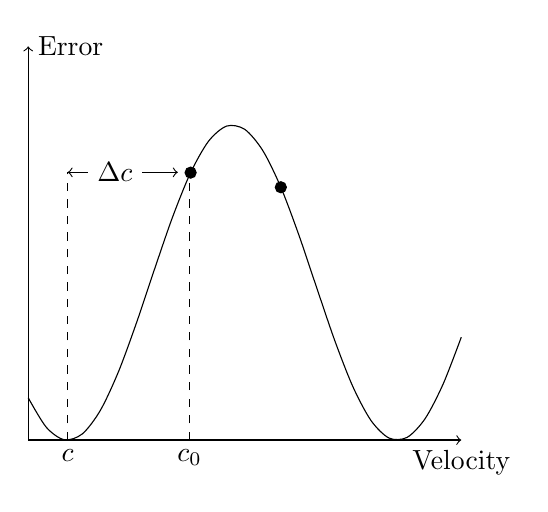
\begin{tikzpicture}[domain=-0.5:5,smooth]
\draw[->] (-0.5,0) -- (-0.5,5.0) node[right] {Error};
\draw[->] (-0.5,0) -- (5,0) node[below] {Velocity};
\node[below] (0,0) {$c$};
\draw[dashed](0,0) -- (0,3.4);
\draw plot[mark=*,mark indices={10,15}] (\x,{2*(1-cos(1.5*\x r))}) ;
\node (x0) at (0.6,3.4){$\Delta c$};
\draw[->] (x0.west) -- (0.0,3.4);
\draw[->] (x0.east) -- (1.4,3.4);
\node[below] at (1.55,0.0) {$c_0$};
\draw[dashed](1.55,0) -- (1.55,3.4);
\end{tikzpicture}
\end{frame}
%-----------------------------------------
\begin{frame}{Initial models for FWI}
%-----------------------------------------

Born approximation holds (Beydoun and Tarantola, 1988)
%
\begin{eqnarray}
 \Delta T < \frac{1}{2f_0}
\end{eqnarray}
%
\begin{itemize}
 \item $\Delta t$ : Traveltime error between model and data
 \item $f_0$: Dominant frequency
\end{itemize}
or (Pratt et al. 2008)
%
\begin{eqnarray}
 \frac{\Delta T}{T}  < \frac{1}{N_{\lambda}}
\end{eqnarray}
%
\begin{itemize}
 \item $N_{\lambda}$ : No of wavelengths
 \item $T$ : Record time
\end{itemize}
\end{frame}
%-----------------------------------------
\begin{frame}{Initial models for FWI}
%-----------------------------------------

Initial model A

\epsfig{file=Fig/fig-8,width=\textwidth} 

%
\end{frame}
%-----------------------------------------
\begin{frame}{Initial models for FWI}
%-----------------------------------------

Initial model B

\epsfig{file=Fig/fig-9,width=\textwidth} 

%
\end{frame}
%-----------------------------------------
\begin{frame}{Initial models for FWI}
%-----------------------------------------
Jian-Bing et al. (2009) for
%
\begin{eqnarray}
  (\omega/c_{0})^2 I < 1,
\end{eqnarray}
%
%
\begin{eqnarray}
  I=\max |\int g(x_r,\omega,x)\frac{\Delta c(x)}{c_{0}(x)} d^3 x|.
\end{eqnarray}
%
$g$ is the acoustic Green's function.

Give max frequencies $\approx 1-10 Hz$ for both model A and B
\end{frame}
%-----------------------------------------
\begin{frame}{WEMVA}
%-----------------------------------------
Wave Equation Migration Velocity Analysis (WEMVA)
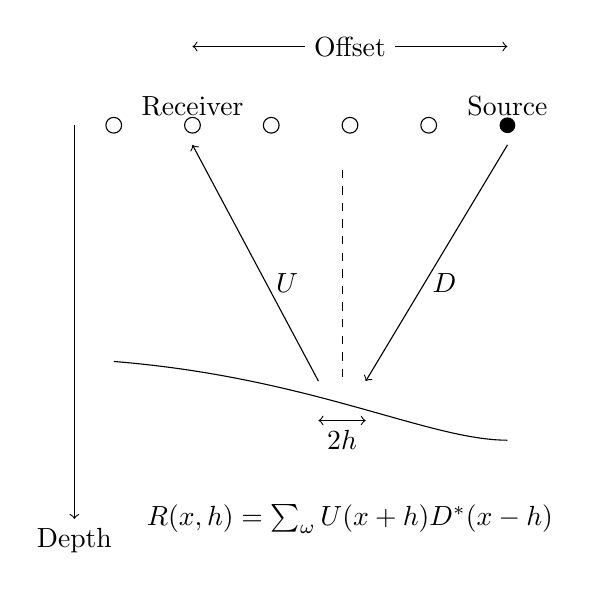
\begin{tikzpicture}
  \draw[->] (-0.5,4.0) -- (-0.5,-1.0) node[below]{Depth} ;
  \draw[<->] (1.0,5.0) -- node[fill=white]{Offset} (5.0,5.0); 
  \fill (5.0,4.0) node[above]{Source} circle (0.1) ;
  \filldraw[white] (0.0,4.0) circle (0.1) ;
  \draw (0.0,4.0) circle (0.1) ;
  \fill[white](1.0,4.0) circle (0.1) ;
  \draw (1.0,4.0) node[above]{Receiver}circle (0.1) ;
  \fill[white] (2.0,4.0) circle (0.1) ;
  \draw (2.0,4.0) circle (0.1) ;
  \fill[white] (3.0,4.0) circle (0.1) ;
  \draw (3.0,4.0) circle (0.1) ;
  \fill[white] (4.0,4.0) circle (0.1) ;
  \draw (4.0,4.0) circle (0.1) ;
  \draw (0.0,1.0) .. controls (2.5,0.8) and (4.0,0.0) .. (5.0,0.0); 
  \draw[->] (5.0,3.75) -- (3.2,0.75); 
  \draw[->] (2.6,0.75) -- (1.0,3.75); 
  \node at (4.2,2.0) {$D$} ;
  \node at (2.2,2.0) {$U$} ;
  \draw[<->] (2.6,0.25) -- node[below]{$2h$} (3.2,0.25) ;
  \node at (3.0,-1.0) {$R(x,h)=\sum_{\omega}U(x+h)D^*(x-h)$} ;
  \node at (2.9,0.65) {$\xx$} ;
  \draw[dashed] (2.9,0.8) -- (2.9,3.5); 
\end{tikzpicture}
\end{frame}
%-----------------------------------------
\begin{frame}{WEMVA}
%-----------------------------------------
Minimize $e_s$ w.r.t $c$ 
\begin{eqnarray}
  e_s = \sum_x \sum_h h^2\left[\frac{\partial R(\xx,\hh)}{\partial z}\right]^2,
                   \label{eq:diffs}
\end{eqnarray}
%
Iterative solution
\begin{eqnarray}
  c=c_0+\Delta c \nonumber\\
  \Delta c \approx \alpha \nabla_c e_s
\end{eqnarray}
%
\begin{itemize}
\item $e_s$ is mainly sensitive to travel-time
\item Low resolution
\item Relies on the Born Approximation
\end{itemize}
\end{frame}
%-----------------------------------------
\begin{frame}{WEMVA}
%-----------------------------------------

Initial model 

\epsfig{file=Fig/fig-8,width=\textwidth} 

%
\end{frame}
%-----------------------------------------
\begin{frame}{WEMVA}
%-----------------------------------------

{Initial model}\\

\epsfig{file=Fig/fig-1,width=7cm} 

{WEMVA 25 iterations}\\

\epsfig{file=Fig/fig-4,width=7cm}

\end{frame}
%
%-----------------------------------------
\begin{frame}{WEMVA}
%-----------------------------------------

Final model 

\epsfig{file=Fig/fig-9,width=\textwidth} 

%
\end{frame}
%-----------------------------------------
\begin{frame}{WEMVA}
%-----------------------------------------

{Exact model}\\

\epsfig{file=Fig/fig-3,width=7cm} 

{WEMVA 25 iterations}\\

\epsfig{file=Fig/fig-4,width=7cm}


\end{frame}
%
%-----------------------------------------
\begin{frame}{Joint Inversion}
%-----------------------------------------
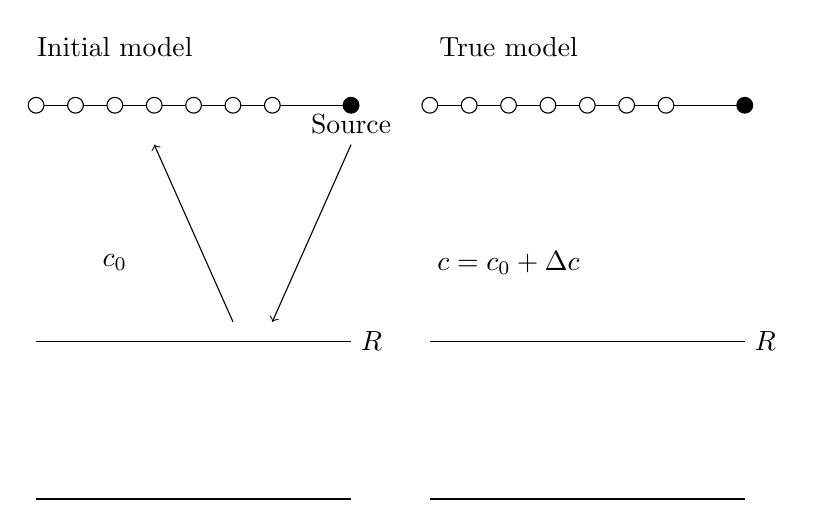
\begin{tikzpicture}
\node[above]  at (1,5.5) {Initial model}; 
\draw (0,5) -- (4,5.0); 
\node[below] at (4,5) {Source};
\draw[->] (4,4.5) -- (3,2.25);
\draw[->] (2.5,2.25 ) -- (1.5,4.5);
\foreach \x in {0,0.5,...,3}
  \draw[fill=white] (\x,5) circle (1mm);
\draw[fill=black] (4,5) circle (1mm);
\node at (1,3) {$c_0$};
\draw (0,2) -- (4,2) node[right]{$R$};
\draw (0,0) -- (4,0); 

\node[above]  at (6,5.5) {True model}; 
\draw (5,5) -- (9,5.0); 
\foreach \x in {5,5.5,...,8}
  \draw[fill=white] (\x,5) circle (1mm);
\draw[fill=black] (9,5) circle (1mm);
\node at (6,3) {$c=c_0+\Delta c$};
\draw (5,2) -- (9,2) node[right]{$R$};
\draw (5,0) -- (9,0); 
\end{tikzpicture}
\end{frame}
%-----------------------------------------
\begin{frame}{Joint Inversion}
%-----------------------------------------

{L2 Error}\\

\epsfig{file=Fig/fig-6,width=7cm} 

%
\end{frame}
%-----------------------------------------
\begin{frame}{Joint Inversion}
%-----------------------------------------

{Differential Semblance Error}\\

\epsfig{file=Fig/fig-7,width=7cm}
%
\end{frame}
%-----------------------------------------
\begin{frame}{Joint Inversion}
%-----------------------------------------
% Minimize joint error $e$ w.r.t $c$ 
\begin{eqnarray}
  e = w_l e_l + w_s e_s
\end{eqnarray}
%
%
\begin{itemize}
\item $w_l, w_s$: Weights 
\item $e_l$: Least-squares Inversion error
\item $e_s$: Differential semblance error 
\end{itemize}
\end{frame}
%-----------------------------------------
\begin{frame}{Joint Inversion}
%-----------------------------------------

{Initial model A}\\

\epsfig{file=Fig/fig-1,width=7cm} 

{WEMVA after 25 iterations}\\

\epsfig{file=Fig/fig-4,width=7cm}
%
\end{frame}
%-----------------------------------------
\begin{frame}{FWI resolution}
%-----------------------------------------

{Initial model from WEMVA}\\

\epsfig{file=Fig/fig-1,width=7cm} 

{FWI Iteration 1 - Initial model =$\Delta c$ }\\

\epsfig{file=Fig/fig-16,width=7cm}

\end{frame}
%-----------------------------------------
\begin{frame}{Joint Inversion}
%-----------------------------------------

{WEMVA model}\\

\epsfig{file=Fig/fig-4,width=7cm} 

{FWI after 25 iterations}\\

\epsfig{file=Fig/fig-5,width=7cm}
%
\end{frame}
%-----------------------------------------
\begin{frame}{Joint Inversion}
%-----------------------------------------

{Exact Model}\\

\epsfig{file=Fig/fig-3,width=7cm} 

{FWI after 25 iterations}\\

\epsfig{file=Fig/fig-5,width=7cm}
%
\end{frame}
%-----------------------------------------
\begin{frame}{Conclusions}
%-----------------------------------------
\begin{itemize}
  \item WEMVA produces low resolution velocity models with
        reasonable good kinematic properties
        from simple initial models 
  \item WEMVA velocity models can be used as initial models for
        FWI to obtain high resolution velocity models
\end{itemize}
%
\end{frame}
%-----------------------------------------
\begin{frame}{Acknowledgements}
%-----------------------------------------
\begin{itemize}
  \item  ROSE consortium, Norwegian Research Coiuncil and Statoil
         for financial support.
  \item E. B. Nilsen for help with Born convergence theory
\end{itemize}
%
\end{frame}
\end{document}
